\documentclass{report}
\usepackage[T1]{fontenc}
\usepackage{color}
\usepackage{amssymb}
\usepackage{pdfpages}
\usepackage{amsmath}
\usepackage{eurosym}
\usepackage{graphicx}
\usepackage{textcomp}
\usepackage{listings}
\usepackage{epigraph}
\usepackage{setspace}
\usepackage{array}
\usepackage{gensymb}
\usepackage{tikz}
\usepackage[some]{background}
\usepackage{geometry}
\usepackage[francais]{babel}


\begin{document}
\renewcommand{\contentsname}{Sommaire}
\renewcommand{\chaptername}{Partie}
\renewcommand{\thechapter}{\Roman{chapter}}

%\usepackage{lmodern}
%\usepackage{xspace}
%\usepackage{hyperref}

\definecolor{sup_strip_color}{rgb}{0.80,0.80,0.80}
\definecolor{inf_strip_color}{rgb}{0.00,0.00,0.00}

\DeclareFixedFont{\bigsf}{T1}{phv}{b}{n}{0.8cm}

\makeatletter                       
\def\printauthor{%                  
    {{\large \@author}}}              
\makeatother

\author{Zohour \textsc{Abouakil} ~\\ Sofia \textsc{Boutahar} ~\\ David \textsc{Courtinot} ~\\ Xiaowen \textsc{Ji} ~\\ Fabien \textsc{Sauce}}

\begin{titlepage}

\newgeometry{left=1cm,right=4cm}
\begin{tikzpicture}[overlay,remember picture]
% the black stripe with the title
\node[
  fill=inf_strip_color,
  anchor=north west,
  text width=\paperwidth,
  text height=2cm,
  text depth=2cm,
  inner xsep=1cm,
  font=\color{white}\bigsf 
  ] 
 at ([yshift=-2.5cm]current page.north west) (blackrect) {Design review - It\'{e}ration 1};
% the khaki stripe
\path[fill=sup_strip_color] 
  (blackrect.north west) rectangle ++(\paperwidth,2.5cm);
\end{tikzpicture}

\vspace*{4.5cm}

\noindent
\begin{minipage}{0.35\linewidth}
    \begin{flushright}
        \printauthor
    \end{flushright}
\end{minipage} \hspace{15pt}
%
\begin{minipage}{0.02\linewidth}
    \rule{1pt}{175pt}
\end{minipage} \hspace{-10pt}
%
\begin{minipage}{0.6\linewidth}
\vspace{5pt}
\newenvironment{test}{\begin{center}}{\end{center}}
\hspace{10pt}
\begin{minipage}{\linewidth} 
Compte-rendu des d\'{e}cisions prises lors des s\'{e}ances de conception du 26/01 au 28/01
\end{minipage}
\end{minipage}

\end{titlepage}
\restoregeometry
\tableofcontents
\chapter{Repr\'{e}sentation AST et CFG}

\paragraph{}
\hspace{4mm}\textnormal{Apr\`{e}s avoir \'{e}tudi\'{e} l'API de Clang, nous sommes arriv\'{e}s \`{a} la conclusion que l'AST comportait bien plus de nuances que ce dont nous avions besoin
pour construire le CFG. En effet, l'atome pour un CFG est ce qu'on appelle g\'{e}n\'{e}ralement une \textit{instruction} tandis que l'instruction la plus simple
donne une repr\'{e}sentation AST compos\'{e}e de plusieurs noeuds. Nous avons par ailleurs jug\'{e} d\'{e}licat de g\'{e}rer \`{a} la fois le parsing et la liaison des noeuds du graphe.
C'est pourquoi nous avons pris le parti de transformer l'AST en une suite d'objets de plus haut niveau que ses noeuds originaux, qui donneront lieux soit \`{a} des blocs
du CFG, soit \`{a} des macro-blocs contenant un sous-graphe.}

\section{Repr\'{e}sentation interm\'{e}diaire de l'AST de Clang}

\subsection{Partie \textbf{Decl}}

\subsection{Partie \textbf{Stmt}}

\paragraph{}
\hspace{4mm}\textnormal{Pour cette premi\`{e}re it\'{e}ration, on ignore totalement la partie objet de C++ pour se concentrer uniquement sur
la partie imp\'{e}rative. En s'inspirant de l'API de Clang, nous sommes arriv\'{e}s au diagramme de classes suivant :}

\begin{center}
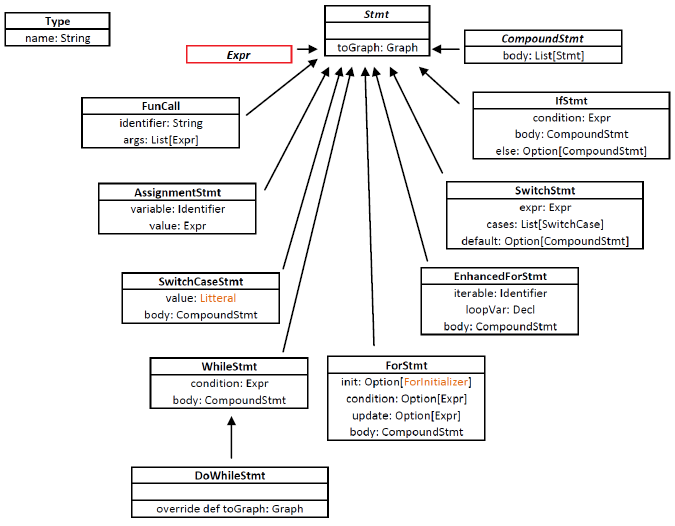
\includegraphics[scale=0.9]{data/stmt.png}
~\\~\\Figure I.1 - Diagramme de classes de la partie (imp\'{e}rative) de \textbf{Stmt}
\end{center}

\paragraph{}
\hspace{4mm}\textnormal{Il est \`{a} noter que notre mod\'{e}lisation ne repr\'{e}sente pas rigoureusement un code C++.  Par exemple, nous n'emp\^{e}chons pas un \textit{if} de contenir d'instruction \textit{break} (parmi d'autres impr\'{e}cisions...).
Nous avons estim\'{e} que ce genre de raffinement compliquerait inutilement la t\^{a}che
sans rien apporter de plus \`{a} l'analyse du CFG. Dans la mesure o\`{u} le code est d\'{e}j\`{a} v\'{e}rifi\'{e} s\'{e}mantiquement par le compilateur Clang et au vu de nos besoins ult\'{e}rieurs,
il appara\^{i}t plus sage de tendre vers un mod\`{e}le simple. Par ailleurs, certaines classes n'ont pas \'{e}t\'{e} clairement d\'{e}finies sur le diagramme pr\'{e}c\'{e}dent, car nous avons volontairement
choisi de les repr\'{e}senter \`{a} part sur le diagramme ci-dessous. Enfin, d'autres classes n'ont pas \'{e}t\'{e} repr\'{e}sent\'{e}es (\textbf{BreakStmt}, \textbf{ContinueStmt} par soucis de lisibilit\'{e}).}

\begin{center}
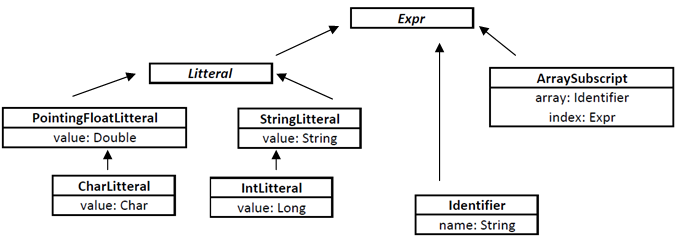
\includegraphics[scale=0.9]{data/expr1.png}
~\\~\\Figure I.2 - Diagramme de classe partiel de la partie \textbf{Expr}
\end{center}

\paragraph{}
\hspace{4mm}\textnormal{Pour finir, nous pr\'{e}sentons un diagramme plus complet pour \textbf{Expr} mais que nous ne sommes pas certains de conserver, sa complexit\'{e} \'{e}tant jug\'{e}e 
superflue pour la nature des algorithmes que nous mettront en place sur ces structures.}

\begin{center}
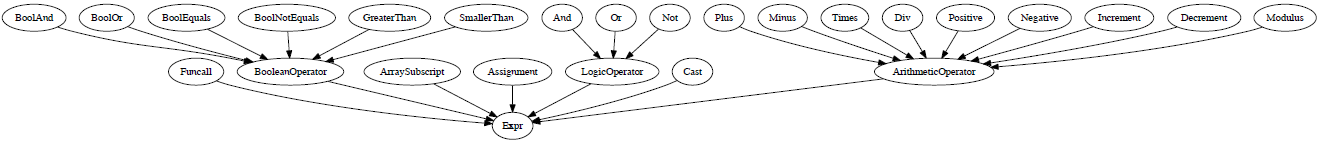
\includegraphics[scale=0.5]{data/expr2.png}
~\\~\\Figure I.3 - Diagramme de classe plus fourni (mais toujours incomplet) de la partie \textbf{Expr}
\end{center}

\subsubsection{Remarques importantes :}

\vspace{4mm}
\begin{itemize}
\item pour repr\'{e}senter fid\`{e}lement le CFG de nos programmes, nous devront tenir compte du m\'{e}canisme de fail-fast dans l'\'{e}valuation des conjonctions/disjonctions.
L'importance de ce m\'{e}canisme pour notre projet est illustr\'{e}e dans la figure suivante.\vspace{1mm}
\item toutefois, l'ordre d'\'{e}valuation des expressions n'\'{e}tant pas sp\'{e}cifi\'{e} en C++ (contrairement \`{a} Java qui \'{e}value de gauche \`{a} droite), nous limiterons ces consid\'{e}rations \`{a} des expressions simples. Nous nous d\'{e}sint\'{e}resserons donc aussi
des expressions (bool\'{e}enes ou non) contenant des sous-expressions \`{a} effet de bord (incr\'{e}mentation, assignations...).\vspace{1mm}
\end{itemize}

\begin{center}
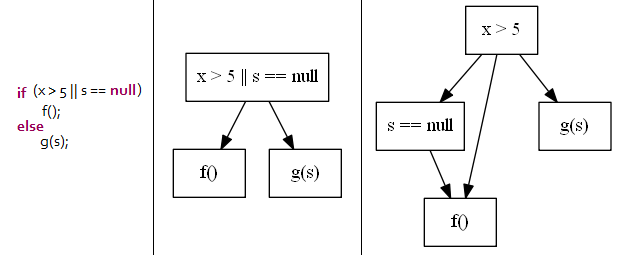
\includegraphics[scale=0.85]{data/fail-fast.png}
~\\~\\Figure I.4 - \`{A} droite, le code consid\'{e}r\'{e}. Au centre, le CFG correspondant \`{a} la non prise en compte du fail-fast et enfin \`{a} droite, prise en compte du fail-fast
\end{center}

\paragraph{}
\hspace{4mm}\textnormal{Comme on peut le constater sur la figure ci-dessus, si l'on cherche \`{a} assurer la propri\'{e}t\'{e} \textit{\og s est toujours initalis\'{e}e lorsque g(s) est appel\'{e}e \fg{}}, le premier CFG ne nous permettra pas de conclure (ou bien il concluera \textbf{true}, \`{a} tort) tandis que le second nous permet de dire qu'il existe des ex\'{e}cutions, selon la valeur de a, 
pour lesquelles $g$ est appel\'{e}e avec un param\`{e}tre non initialis\'{e} (si l'on admet que le fils gauche repr\'{e}sente toujours un test r\'{e}ussi et que le fils droit repr\'{e}sente un test \'{e}chou\'{e}).}

\section{AST to CFG}

\chapter{Model checking}

\end{document}
